\documentclass{standalone}
\usepackage{tikz}
\usetikzlibrary{shapes,arrows,positioning,fit,backgrounds}

\begin{document}
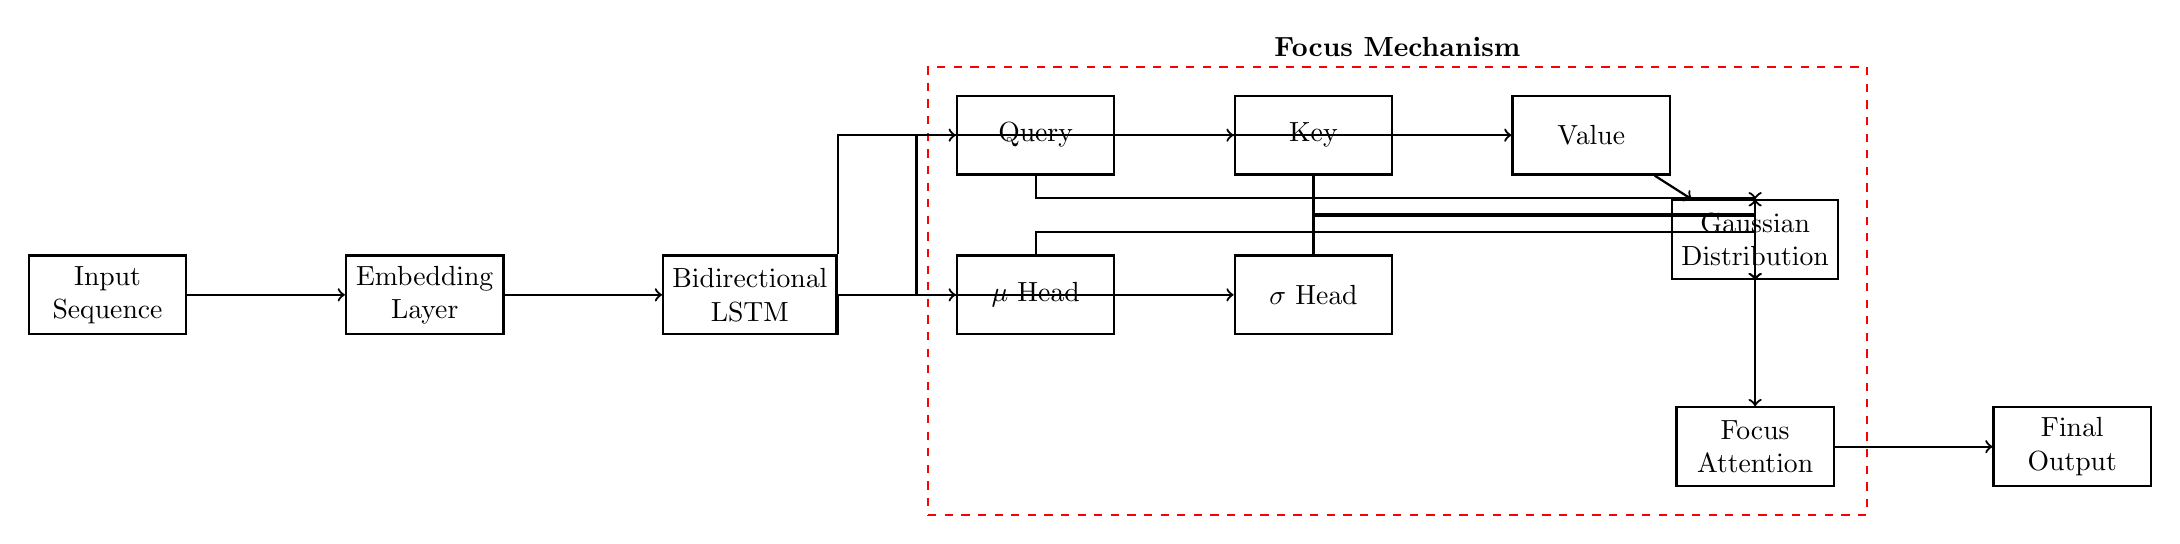
\begin{tikzpicture}[
    node distance=2.0cm,
    box/.style={rectangle,draw,minimum width=2cm,minimum height=1cm,align=center},
    arrow/.style={->,thick},
    thick
]

%--- Nodes: Input to LSTM ---%
\node[box] (input) {Input\\Sequence};
\node[box,right=of input] (embed) {Embedding\\Layer};
\node[box,right=of embed] (lstm) {Bidirectional\\LSTM};

%--- Focus Mechanism grouping ---%
% Place the Q, K, V across the top row of the focus mechanism
\node[box,above right=1.0cm and 1.5cm of lstm] (query) {Query};
\node[box,right=1.5cm of query] (key) {Key};
\node[box,right=1.5cm of key] (value) {Value};

% Place mu, sigma across the bottom row of the focus mechanism
\node[box,below=1.0cm of query] (mu) {$\mu$ Head};
\node[box,below=1.0cm of key] (sigma) {$\sigma$ Head};

% Gaussian distribution in the middle-right
\node[box,below right=0.3cm and 0.0cm of value, align=center] (gaussian) {Gaussian\\Distribution};

% Focused attention output below gaussian
\node[box,below=1.6cm of gaussian] (attention) {Focus\\Attention};

% Final output to the right of attention
\node[box,right=of attention] (output) {Final\\Output};

%--- Draw arrows for the main flow (Input -> Embedding -> LSTM -> Focus Mechanism -> Output) ---%
\draw[arrow] (input) -- (embed);
\draw[arrow] (embed) -- (lstm);

%--- LSTM outputs feeding into Focus Mechanism: Q, K, V, mu, sigma ---%
\draw[arrow] (lstm.north east) |- (query.west);
\draw[arrow] (lstm.north east) |- (key.west);
\draw[arrow] (lstm.south east) |- (mu.west);
\draw[arrow] (lstm.south east) |- (sigma.west);
\draw[arrow] (lstm.east) -- ++(1.0,0) |- (value.west);

%--- Edges within Focus Mechanism ---%
\draw[arrow] (query) -- ++(0,-0.8) -| (gaussian.north);
\draw[arrow] (key) -- ++(0,-1.0) -| (gaussian.north);
\draw[arrow] (value) -- (gaussian);

\draw[arrow] (mu) -- ++(0,0.8) -| (gaussian.south);
\draw[arrow] (sigma) -- ++(0,1.0) -| (gaussian.south);

%--- Gaussian -> Focus Attention -> Final Output ---%
\draw[arrow] (gaussian) -- (attention);
\draw[arrow] (attention) -- (output);

%--- Dashed box around the Focus Mechanism ---%
\begin{scope}[on background layer]
\node[rectangle,draw=red,dashed,thick,
      fit=(query)(key)(value)(mu)(sigma)(gaussian)(attention),
      inner sep=10pt,
      label={[align=center]above:\textbf{Focus Mechanism}}] {};
\end{scope}

\end{tikzpicture}
\end{document}
